% ==============================================================================
% 01_introduction.tex
% Phụ trách: Thành viên 1 (Cơ sở nghiên cứu, phương pháp và dữ liệu)
% ==============================================================================
% TODO [Thành viên 1]:
% - Bối cảnh RAG, vai trò trung tâm của chunking trong việc định hình embedding và retrieval.
% - Đặc điểm đặc thù của tài liệu kỹ thuật Markdown (heading hierarchy, fenced code blocks, callouts).
% - Hạn chế của việc coi tài liệu như văn bản phẳng (flat text).
% - Vấn đề nghiên cứu cốt lõi: Bảo toàn cấu trúc tài liệu có thực sự cải thiện hiệu quả RAG hay không?
% - Ba câu hỏi nghiên cứu (RQ1: Retrieval Ranking, RQ2: Evidence Recovery, RQ3: Answer Quality).
% - Ba đóng góp chính của đề tài.
% ==============================================================================

\section{Introduction}
\label{sec:introduction}

Retrieval-Augmented Generation \citep[RAG;][]{lewis2020retrieval} has become the dominant architectural framework for grounding Large Language Models (LLMs) on private, domain-specific, and rapidly updated knowledge bases. 
In software development ecosystems, developer portals and technical documentation serve as the definitive source of truth. 
These technical corpora are almost universally formatted in structured Markdown, featuring rich syntactic elements such as multi-tiered heading hierarchies (\texttt{\#}, \texttt{\#\#}, \texttt{\#\#\#}), fenced code blocks with explicit language tags, structured tables, and informational callout admonitions.

At the core of every RAG system lies document chunking---the process of partitioning continuous source texts into discrete, indexed units. 
Despite the sophisticated structure of technical Markdown, prevailing industrial pipelines treat documents as flat, unstructured text streams, segmenting them via arbitrary character or token counts. 
This flat text assumption introduces critical syntactic and semantic failure modes:
\begin{itemize}
    \item \textbf{Syntactic Bisection:} Arbitrary windowing indiscriminately severs code blocks, leaving dangling delimiters or splitting function calls away from their type definitions and import statements.
    \item \textbf{Contextual Disconnect:} Subsections and explanatory paragraphs lose their parent structural ancestry, producing embeddings that are semantically ungrounded.
    \item \textbf{Diluted Evidence Recovery:} When evidence for a technical query spans multiple related sub-blocks, naive splitting scatters these fragments across unrelated chunks.
\end{itemize}

\begin{figure*}[t]
    \centering
    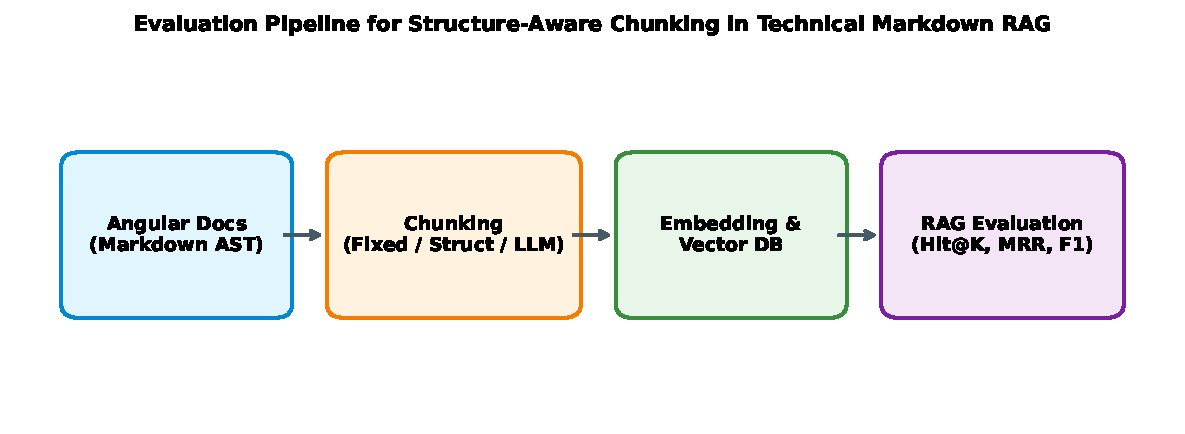
\includegraphics[width=0.92\textwidth]{figures/pipeline_placeholder.pdf}
    \caption{Overview of the controlled evaluation framework: 384 Angular technical Markdown documents are segmented under three chunking strategies (Fixed-size, Structure-aware, Prompt-based), indexed into dense embeddings, and evaluated under identical retrieval and context budgets against 140 expert-curated QA pairs.}
    \label{fig:pipeline_overview}
\end{figure*}

\subsection{Research Problem and Questions}
These pervasive limitations raise a fundamental empirical question: \textit{Does explicitly preserving document structure during chunking genuinely improve end-to-end RAG performance, or does it introduce new structural trade-offs?} 
To rigorously answer this question, we formulate three targeted Research Questions (RQs):
\begin{itemize}
    \item \textbf{RQ1 (Retrieval Ranking):} How does structure-aware chunking compare to fixed-size sliding windows and prompt-based chunking in early-stage retrieval ranking (Hit@$K$, MRR)?
    \item \textbf{RQ2 (Evidence Recovery):} To what extent does preserving heading hierarchy and atomic block boundaries improve the retrieval coverage of complete gold evidence spans (Evidence Coverage, All-Evidence-Retrieved Rate)?
    \item \textbf{RQ3 (Answer Generation Quality):} How do the resulting chunk granularities and retrieval contexts impact downstream response fidelity (Token Precision, Token Recall, and Token F1)?
\end{itemize}

\subsection{Main Contributions}
This research delivers three core contributions to the study of RAG on technical corpora:
\begin{enumerate}
    \item \textbf{A Standardized Technical Documentation Benchmark:} We build and release an expert-validated benchmark based on 384 Angular Markdown documents, containing 140 curated QA pairs stratified across three difficulty levels (60 easy, 40 medium, 40 hard) with 233 granular evidence spans completely decoupled from chunk boundaries.
    \item \textbf{Controlled Comparative Framework:} We systematically benchmark three representative chunking paradigms---Fixed-size, Structure-aware (AST), and Prompt-based (LLM with local validation)---under identical embedding, retrieval budget (2,048 tokens), and context budget (4,096 tokens) constraints.
    \item \textbf{Empirical Trade-off Characterization:} We identify and explain key trade-offs between early-rank retrieval precision and broad evidence recall, proving that no single chunking strategy dominates across all RAG objectives and providing actionable architectural guidelines for practitioners.
\end{enumerate}
